\documentclass[border=10pt]{standalone}
\usepackage{pgfplots}
\usepgfplotslibrary{colormaps}
\pgfplotsset{compat=1.18}

\begin{document}
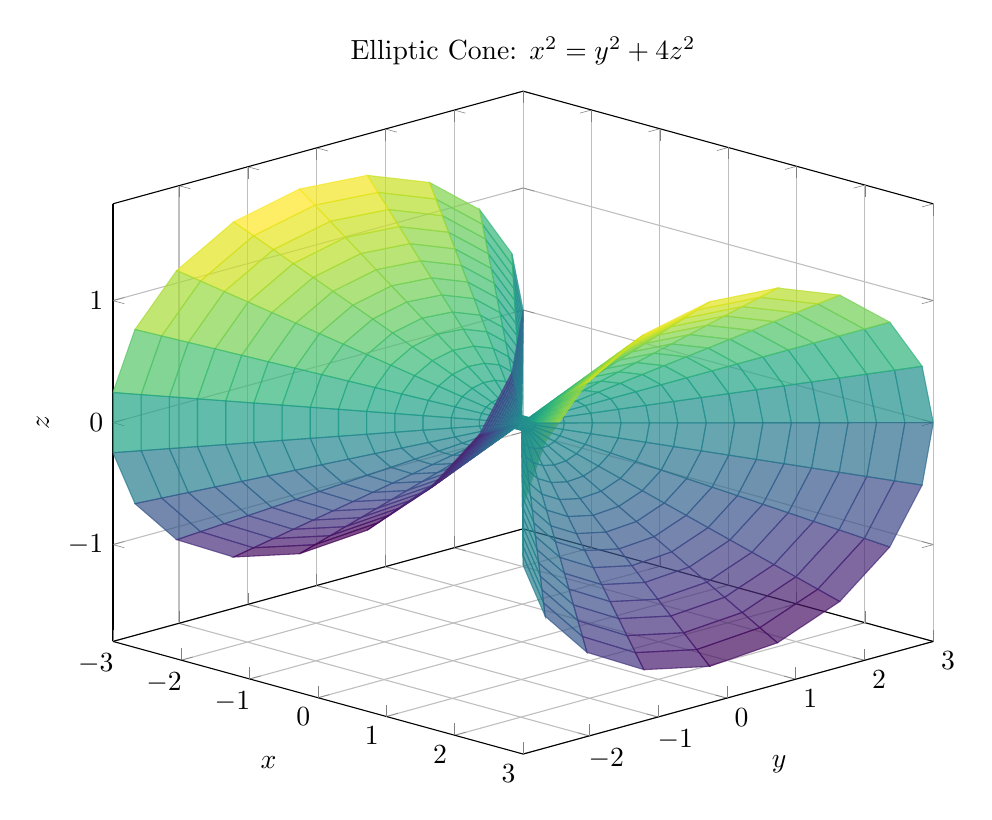
\begin{tikzpicture}
\begin{axis}[
    view={45}{20},
    xlabel={$x$},
    ylabel={$y$},
    zlabel={$z$},
    title={Elliptic Cone: $x^2 = y^2 + 4z^2$},
    colormap/viridis,
    grid=major,
    width=12cm,
    height=10cm,
    domain=-3:3,
    y domain=0:2*pi,
    samples=30,
    samples y=20,
]
% Parametric surface: x = x, y = |x|*cos(theta), z = |x|/2*sin(theta)
\addplot3[surf, shader=flat corner, opacity=0.7] 
    ({x}, {abs(x)*cos(deg(y))}, {abs(x)/2*sin(deg(y))});
\end{axis}
\end{tikzpicture}
\end{document}
